***(General notes/questions
\begin{itemize}
\item I wasn't sure how much to include about the Cisneros thesis and BEAU.  It's true that it informed how I handled the pebbles - knowing they move in slug flow, for example - but I didn't use any of the lattice models that thesis did, and while I would like to explore the fuel burnup a bit more in depth next, I'm not sure that fits this thesis right now
\item I think we talked about the fact that i can afford to go into more detail on PBMR because of the long time spent on it, but I'll wait for the first review to add anything
\item I was going to include a brief section on some micro reactor designs from recent years, but I don't really have a set method for selecting which designs and articles I should mention, and I don't want it to seem random or hodge-podge.  (if I do make a few paragraphs about this, would it be appropriate to reference Roberto's thesis? technically I think it definitely fits, I mean more in the context of being polite/proper)
\end{itemize}
)***
\section{Computational Model}

\subsection{Serpent}

Serpent 2 is "a multi-purpose three-dimensional continuous-energy Monte Carlo particle transport code" \cite{noauthor_serpent_nodate} from the VTT Technical Research Center of Finland.  The first iteration, Serpent 1, began development in 2004.  The development of Serpent 2 is presently ongoing.  Serpent 2 has three main applications: traditional reactor physics, coupled multi-physics, and neutron and photon transport.  In order to create and model complex geometries, Serpent uses constructive solid geometry (CSG), which defines homogeneous material cells using user-defined universes, cells, lattices, and specially-defined nested objects to define particle and pebble geometries.  

Using these special objects and the particle dispersal routine in Serpent, TRISO particles and pebble bed reactors can be modeled.  The particle dispersal routine works by first establishing a user defined container for the particles, such as a cylinder.  The user then defines the size of the particles - all of which are assumed to be perfect spheres - and either the number of particles, or the packing fraction of particles in the container.  Serpent then randomly generates coordinates for the center of the dispersed particles.  For each location, Serpent checks that the entire particle is inside the container, and that it does not overlap with any other particles.  It then prints a text file with the coordinates of each particle center, along with the radii and the universe they're located in.  Serpent has been tested with up to 60 million individual particles.

Physics are based on a combination of classical kinematics, ENDF reaction laws, and random sampling.  For particle transport, Serpent uses surface tracking and Woodcock-delta tracking.  For material data, Serpent uses ACE format libraries for microscopic cross sections, and pre-generates macroscopic cross sections before beginning transport.  To further speed-up calculations, Serpent uses a unionized energy grid.

Serpent has been validated against MCNP, and validation is ongoing for radiation shielding and criticality safety analysis.  While the differences between Serpent and other Monte Carlo codes are generally small, Serpent experiences the same issues validating its results as other Monte Carlo programs, related to small differences in data libraries.

\subsection{Experience from BEAU}

BEAU, or Burnup Equilibrium Analysis Utility, was developed by Dr.Cisneros to model depletion and multiple burnup states for a continuously refueled molten-salt PBMR.  While a full examination of all possible pebble burnups and compositions is not the target of this work, the experience in modeling a pebble bed reactor was invaluable.  In particular, the development of the Mark 1 PB-FHR (pebble-bed fluoride salt cooled high temperature reactor), the methods to model pebbles, and the flow of pebbles through the core, informed the Sangamon20 design.


\section{The High Temperature Gas Cooled Reactor: Beginnings and Concepts}

High temperature gas cooled reactors, or HTGRs, are one of the more commonly seen Generation IV reactor designs.  It most often uses helium as a coolant, and graphite as a moderator in thermal designs.  Fuel is in the form of tristructural-isotropic, or TRISO particles.  TRISO particles use a small kernel of fuel, less than half a millimeter across, surrounded by layers of carbon and silicon carbide to protect the fuel kernel and prevent the leakage of radioisotopes ***(would it also be accurate to say the layers provide moderating material?  I know that graphite is a great moderator, but I would think the main purpose is safety and to prevent leaching, and moderation is really in the graphite the particles are embedded in)***.  These TRISO particles are then embedded in graphite to form a usable fuel element.  In prismatic HTGRs, the graphite is in the shape of hexagonal columns.  In pebble-bed reactors, the graphite is in the shape of spheres, around the size of a billiard ball.  Many of these pebbles are loaded into the core, and slowly move through the bottom in a manner not dissimilar to grain in silos.

HTGRs, however, are not a new concept.  Preliminary concepts for a gas-cooled reactor were created as early as 1942.  Farrington Daniels - more commonly known for work in chemistry and solar power technology - is attributed with establishing the first theoretical designs.  A professor from the University of Wisconsin, Professor Daniel's work with Oak Ridge National Laboratory (ORNL) nailed-down the most basic characteristics of the HTGR.  The choice of helium for coolant, graphite for moderator, the direct gas turbine cycle, and the use of uranium or thorium carbides for fuel all came from his work \cite{simnad_early_1991}.

Professor Daniels recognized early on the importance of a small power-producing unit with low initial costs and ease of transport in developing nations - a sentiment that has resurfaced in recent years in the designs for small modular reactors.  Daniels' first design was for a simple high-temperature pebble pile.  A little over a decade later, improvements to turbine technology prompted him to propose a direct-cycle helium cooled reactor.  However, before any construction could start, the Atomic Energy Commission opted to support Light Water Reactor (LWR) technology instead \cite{simnad_early_1991}.

\begin{figure}[h!]
\centering
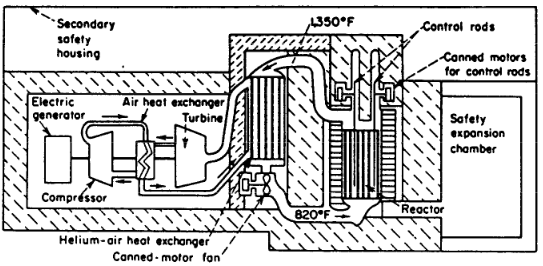
\includegraphics[width=0.6\linewidth]{figures/daniels-1}
\caption{Side-View of the 1955 Daniels' Concept, \cite{simnad_early_1991}}
\label{fig:daniels-1}
\end{figure}
\begin{figure}[h!]
\centering
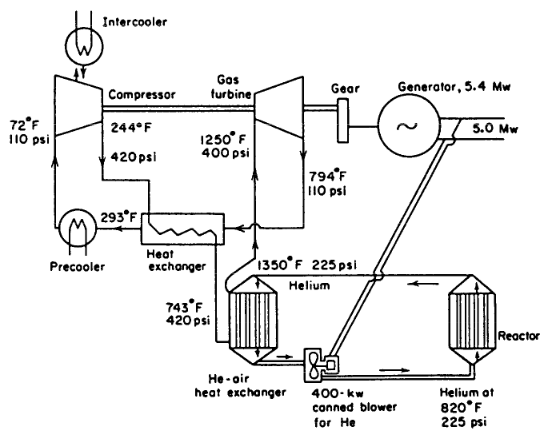
\includegraphics[width=0.6\linewidth]{figures/daniels-2}
\caption{Diagram of Coolant Flow in the 1955 Daniel's Concept, \cite{simnad_early_1991}}
\label{fig:daniels-2}
\end{figure}

Figures \ref{fig:daniels-1} and \ref{fig:daniels-2} show the design of the 1955 design proposed by Professor Daniels.  Like many modern modular reactor plant designs, Professor Daniels suggested that the reactor be mostly underground.  A key difference between the Farrington Daniels designs and modern HTGRs is the fuel form.  While modern designs use TRISO particles embedded in graphite, the Daniels' design uses solid graphite blocks, with channels for both coolant and fuel.  Within the fuel channels, fuel was loaded in either a pellet or cartridge form, both a mixture of 10$\%$ uranium dicarbide and graphite powder.  In addition to these fuel channels, the design included an outer ring of graphite reflector in which thorium was used to breed U-233.  Control rods were made of boron-containing molybdenum.  Additional safety rods made of the same were held above the core by steel wires that would melt in the case of an accident, dropping the safety rods into the core \cite{simnad_early_1991}.

\section{Earliest Operational HTGRs}

The earliest operational HTGRs were first started in the 1960s.  The AVR, from Germany, Dragon, operating in the UK, and Peach Bottom 1, which operated in the US \cite{beck_high_nodate}.

\subsection{Dragon}

The Dragon prismatic HTGR was a test reactor operated in Winfrith, UK, from 1964 to 1975, making it the oldest of the reactors discussed in this chapter.  It operated at inlet and outlet temperatures of 350\textdegree  C and 750\textdegree  C and a power of 20MWt \cite{beck_high_nodate}.  Dragon's main purpose was to test reactor materials, with an emphasis on fuels.  It originally used uranium and thorium as fuel, but switched to a purely uranium-based fuel with a lower enrichment later in life.  The fuel elements themselves were similar in shape to the Daniels' design - hexagonal prisms with fuel rod channels.

Contrary to the fuel philosophy seen today, Dragon originally allowed fission products to be released from fuel elements into the circulating helium coolant.  The fission products would then be purged from the helium.  However, Dragon later switched to a coated-particle fuel when it became clear that having such large fission product releases would be difficult to manage \cite{simnad_early_1991}.

\subsection{Peach Bottom 1}

Peach Bottom 1 operated from 1966 to 1974, by the Philadelphia Electric Company.  It was the first operational HTGR in the US, and the first to produce electric power.  It was slightly larger than Dragon, at a nameplate capacity of 115 MWt/40MWe and a slightly lower operating temperature range at 327\textdegree  C to 700\textdegree  C inlet to outlet \cite{beck_high_nodate}.  Like Dragon, Peach Bottom 1 was a prismatic reactor, however, Peach Bottom used coated uranium and thorium carbide particles from the beginning.  The original fuel used a single coating of pyrolytic carbon.  However, after multiple fuel failures, Peach Bottom upgraded to bistructural isotropic, or BISO, fuels by adding an additional layer.  Peach Bottom would later upgrade the fuel once again by adding a silicon carbide layer, forming TRISO particles \cite{beck_high_nodate}.  One operational benefit of upgrading to TRISO particles from BISO particles was that the superior fission product retention meant that Peach Bottom 1 could remove the helium purging systems.  In addition to the inner fuel region, Peach Bottom, like the Daniels' design, bred U-233 in an outer region using thorium.

Beyond changing the number and materials for fuel coatings, the experiences in Peach Bottom 1 helped to develop HTGR fuel elements.  Operators saw that by using the graphite moderating material to dilute the fuel, the fuel could be diluted further compared to other diluents.  This of course has the advantage of saving fuel material, but also improved heat transfer and reduced radiation damage.  Additionally, operational experience showed that, in order to prevent the creation and buildup of U-236 and Np-237, which are poisons, the U-235 and U-233 should be kept separate \cite{simnad_early_1991}.

In the end, Peach Bottom 1 closed when it was determined to be uneconomical.

\subsection{AVR}

The Arbeitsgemeinschaft Versuchsreaktor (AVR) was an experimental pebble-bed reactor operated in the Jülich Research Center from 1967 to 1988.  It had a capacity of 46 MWt/15MWe, with inlet and outlet temperatures of 275\textdegree  C and 950\textdegree  C \cite{beck_high_nodate}.  In fact, the AVR reached the highest operating temperatures of any commercial nuclear plant.  Like the others in this early time period. the AVR used a combination of uranium and thorium fuels, though the AVR began with BISO particles.  The core held around 100,000 graphite pebbles, almost a third of which had fuel in them.

Despite not being built for experimental purposes, the AVR still housed many experiments that improved our body of knowledge in HTGR technology.  During the first few years of its life, the goal of the AVR was to demonstrate that it was a reliable technology.  After this inital period, the AVR could shift to allowing various experiments.

A step was to show that the reactor could operate safely, could control the core power and temperatures and safely shut down and remain sub-critical for long periods of time.  This proved to be quite the undertaking, as the AVR shifted from highly enriched to low enriched fuel over time, which caused a large variety in fuel pebble compositions, on top of the range of compositions inherent to a multi-pass pebble cycle.

The AVR also provided data to validate models of pebble-bed reactors, and conducted an experiment to better characterize the radial distribution of temperatures in the core.  A number of marked pebbles were loaded into the core, each housing a series of wires that would melt at a certain temperature, the lowest being 655\textdegree  C, the highest 1280\textdegree  C.  The pebble positions were tracked based on pebble flow data, and when the spheres were ejected, the were examined to determine what temperatures the pebbles had experienced.  Despite the outlet temperature being determined to be 950\textdegree  C, multiple pebbles experienced a temperature greater than or equal to the 1280\textdegree C maximum temperature in the melt wires.  It was noted that these pebbles went through a zone with a spike in local power density \cite{noauthor_results_1990}.

The AVR also demonstrated the inherent safety of HTGR reactors in accident scenarios by purposefully causing failure of active cooling system "accidents".  In the first, the the coolant blowers were shutoff, and no shutdown rods were inserted while operating at full power.  The operators additionally shut the main circuit valves to prevent natural circulation to regions outside the active core.  Overall, the changes to core temperatures were unremarkable.  The hottest regions cooled, while the coldest regions warmed up.  Additionally, due to negative temperature feedback coefficients, the reactor power immediately declined in response to the "accident".  The temperature slowly rose to 2 MW again over 24 hours, only to level out around 300 kW.  A further test provided data on loss of coolant and depressurization accidents.  As before, the core temperature changes were not particularly drastic.  The upper core region was seen cooling, while the lower, originally cooler core region slowly rose in temperature.  This experiment's data was used to validate HTGR computer models, which allowed the results to be aid in the analysis of other HTGRs \cite{noauthor_results_1990}.

Beyond accident safety, the AVR allowed for testing and demonstration of the safety qualities of TRISO and BISO fuel elements, especially relating to high temperature tolerance and fission product retention.  Inital tests were conducted with BISO based pebbles, then later transitioned to TRISO, then low-enriched TRISO pebbles.  The TRISO-LEU pebbles were shown to have good fission product retention compared to their BISO-based predecessors, based on the results of sampling the activity of the circulating helium to to the presence of released fission products.  Beyond radioisotopes being directly released into the coolant gas, the AVR also showed that in order to accurately characterize the source term of am HTGR pebble bed reactor, one must take the dust from the pebbles into account.  Dust from the pebbles bumping and scraping against each other was found deposited on reactor surfaces in the primary loop.  It was found that 60 kg of dust had accumulated by the end of the reactor's life, which averages to 3 kg of dust each year.  Measurements of specific activity in the dust showed that the activities of Cs-137, Cs-134, I-131, Sr-90, and Co-60 were on the order of $10^6 \frac{Bq}{g}$.  Even though there is relatively little dust, the activity of this dust is fairly high, especially compared to the activity of the coolant gas \cite{noauthor_results_1990}.

***(I'm going to include here the two tables comparing the activities of the coolant gas and dust activities.  However, the one for gas is (reasonably) by volume, while the dust is by mass.  Should I use the density of helium at operating temperature to convert the gas activity to be in Bq/g, and make a new table (citing my source), or leave as-is?)***

\begin{figure}[h!]
\centering
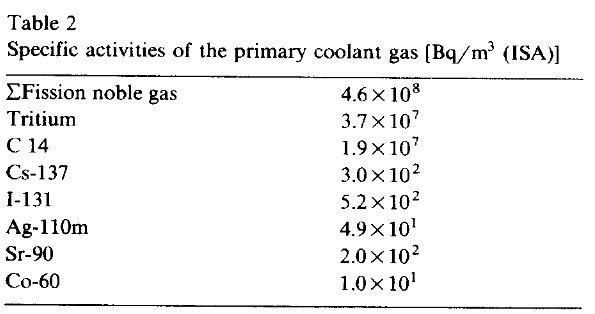
\includegraphics[width=0.7\linewidth]{figures/gas-act-tab}
\caption{Helium Coolant Specific Activities \cite{noauthor_results_1990}}
\label{fig:gas-act-tab}
\end{figure}
\begin{figure}[h!]
\centering
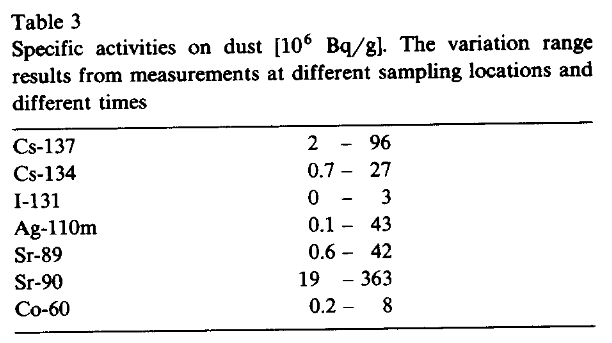
\includegraphics[width=0.7\linewidth]{figures/dust-act-tab}
\caption{Pebble Dust Specific Activities \cite{noauthor_results_1990}}
\label{fig:dust-act-tab}
\end{figure}


\section{Modern HTGRs}

\subsection{PBMR}

The PBMR is a South African pebble bed HTGR design.  While it did not ultimately make it to construction, its design has offered invaluable insight to later HTGR pebble bed designs.  The PBMR is largely based on the German High Temperature Reactor (HTR) designs, and has a nameplate thermal power of 400 MW, with inlet-outlet temperatures of 500 \textdegree C to 900 \textdegree C.  It is a modular design, with each unit containing a graphite moderated, helium-cooled core housed in a steel pressure vessel.  In accident scenarios, the PBMR would rely on passive safety features using conduction and convection to provide cooling.

\begin{figure}[h!]
\centering
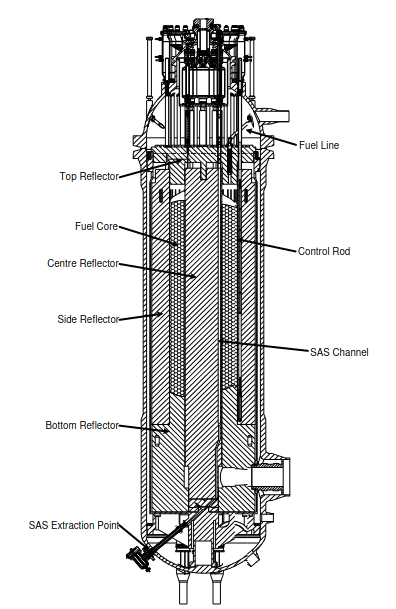
\includegraphics[width=0.5\linewidth]{figures/pbmr-v-cross-sect}
\caption{PBMR Schematic: Vertical Cross-section \cite{venter_pbmr_2005}}
\label{fig:pbmr-v-sect}
\end{figure}

Each core unit would hold around half a million pebbles, which used LEU based TRISO particles as the fuel form.  These TRISO particles are pressed into a 2.5cm radius graphite sphere, which then has an additional 0.5 cm thick layer of graphite pressed around it, to form a 3.0 cm radius pebble - around the size of a billiard ball.  The pebbles would undergo a six-pass multi-pass cycle to reach a target end burnup of 92,000 $\frac{MWd}{tU}$ \cite{venter_pbmr_2005}. 

\subsection{Next Generation Nuclear Plant (NGNP}

Like the PBMR, the NGNP did not make it to construction.  However, the work in analyzing reactor designs and materials is still applicable to other work.  The NGNP project downselected its design choices to two models - a prismatic HTGR and a pebble-bed HTGR.  While the NGNP project eventually opted for the Areva prismatic HTGR design \cite{noauthor_areva_nodate} due to reasons related to pebble costs, it was noted that, technologically speaking, there was no inherent advantage or disadvantage bewteen the two technologies \cite{inl_basis_2011}.

Even though the reactor didn't make it to construction or operation, the NGNP project, and the resulting white papers, have provided an invaluable licensing example for generation IV reactors with the NRC.  As much of the current NRC guidelines are based upon LWR technology, work towards validating HTGR materials still has to be developed \cite{lommers_ngnp_2012}.

\subsection{X-energy}

Based on experience working on the PBMR project, the X-energy Xe-100 is a 200 MWt HTGR pebble-bed SMR.  It is similar in design to all of its predecessors, featuring LEU TRISO particle fuel in 3.0 cm radius pebbles.  While the Xe-100, or similar demonstration plant, has not been built as of this publication, the project ***(company?  work?  design?)*** is still ongoing.  It is this reactor, and by extension, the PBMR, that the micro-reactor described in this thesis is most heavily influenced by.

The Xe-100 uses approximately 220,000 pebbles in a six-pass cycle, and fuel pebbles identical to the ones intended for the PBMR \cite{harlan_x-energy_2018}.  However, while the number of passes is the same, the target end burnup for the pebbles is higher, at 160,000 $\frac{MWd}{tU}$ \cite{agnihotri_intrinsically_2017}.  Another key difference from the PBMR beyond size is the lack of central reflector.

While the Xe-100 has not been built, there have been studies conducted by ORNL providing data on the production and material properties of the PBMR-type fuel pebble.
